% ch3p5_002: Using styles
% Define styles
\documentclass[tikz, border=10pt]{standalone}

\usepackage{tikz}
\usetikzlibrary{arrows.meta, decorations.pathmorphing, backgrounds, positioning, fit, petri}

\begin{document}
	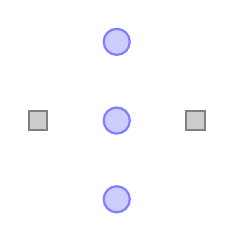
\begin{tikzpicture}[
		place/.style={circle, draw=blue!50, fill=blue!20, thick},
		transition/.style={rectangle, draw=black!50, fill=black!20, thick}
		]
		\node at (0, 2) [place] {};
		\node at (0, 1) [place] {};
		\node at (0, 0) [place] {};
		\node at (1, 1) [transition] {};
		\node at (-1, 1) [transition] {};
	\end{tikzpicture}
\end{document}